\documentclass[a4paper]{jpconf}
\usepackage{graphicx}
\usepackage{color}
\usepackage{array}
\usepackage{enumerate}

\begin{document}
\title{The production deployment of IPv6 on WLCG}

\author{J Bernier$^1$, S Campana$^2$, K Chadwick$^3$, J Chudoba$^4$, 
        A Dewhurst$^5$, M Eli\'a\v s$^4$, S Fayer$^6$, T Finnern$^7$,
        C Grigoras$^2$, B Hoeft$^7$, T Idiculla$^5$, D P Kelsey$^5$,  
        F L\'opez Mu\~noz$^9$, E Macmahon $^{10}$, E Martelli$^2$, R Nandakumar$^5$, 
        K Ohrenberg$^7$, F Prelz$^{11}$, D Rand$^6$, 
        A Sciab\`a$^2$, U Tigerstedt$^{12}$, R Voicu$^{13}$, 
        C J Walker$^{14}$ and T Wildish$^{15}$}

\address{$^1$ IN2P3 Computing Centre, Boulevard du 11 Novembre 1918, F-69622 Villeurbanne Cedex, France}
\address{$^2$ CERN, CH-1211 Gen\`eve 23, Switzerland}
\address{$^3$ Fermi National Accelerator Laboratory, Batavia, Il 60510, U.S.A.}
%\address{$^3$ Institute of High Energy Physics, 19B Yuquanlu, Shijingshan District, 100049 Beijing, China} 
\address{$^4$ Institute of Physics, Academy of Sciences of the Czech Republic Na Slovance 2 182 21 Prague 8, Czech Republic}
\address{$^5$ STFC Rutherford Appleton Laboratory, Harwell Oxford, Didcot, Oxfordshire OX11 0QX, United Kingdom}
\address{$^6$ Imperial College London, South Kensington Campus, London SW7 2AZ, United Kingdom}
\address{$^7$ Deutsches Elektronen-Synchrotron, Notkestra\ss e 85, D-22607 Hamburg, Germany}
\address{$^8$ Karlsruher Institut f\"ur Technologie, Hermann-von-Helmholtz-Platz 1, D-76344 Eggenstein-Leopoldshafen, Germany}
\address{$^9$ Port d'Informaci\'o Cient\'ifica, Campus UAB, Edifici D, E-08193 Bellaterra, Spain}
\address{$^{10}$ The University of Oxford, Denys Wilkinson Building, Keble Road, Oxford OX1 3RH, United Kingdom}
\address{$^{11}$ INFN, Sezione di Milano, via G. Celoria 16, I-20133 Milano, Italy}
\address{$^{12}$ CSC Tieteen Tietotekniikan Keskus Oy, P.O. Box 405, FI-02101 Espoo}
\address{$^{13}$ California Institute of Technology, Pasadena, Ca 91125, U.S.A.}
\address{$^{14}$ Queen Mary University of London, Mile End Road, London E1 4NS, United Kingdom}
\address{$^{15}$ Princeton University, Jadwin Hall, Princeton, NJ 08544, U.S.A.}

\ead{david.kelsey@stfc.ac.uk, ipv6@hepix.org}

\begin{abstract}
The world is rapidly running out of IPv4 addresses; the number of IPv6 end systems connected
to the internet is increasing; WLCG and the LHC experiments may soon have access to worker
nodes and/or virtual machines (VMs) possessing only an IPv6 routable address. The HEPiX
IPv6 Working Group ({\tt http://hepix-ipv6.web.cern.ch/}) has been investigating, testing and
planning for dual-stack services on WLCG for several years. Following feedback from our
working group, many of the storage technologies in use on WLCG have recently been made
IPv6-capable. The worldwide HEP computing community now needs to deploy dual-stack
IPv6/IPv4 services on WLCG to allow such use of IPv6-only resources.
This paper will present the IPv6 requirements, tests and plans of each of the four LHC
experiments together with the tests performed both on the IPv6 test-bed and in targeted use
of WLCG production services. This is primarily aimed at IPv6-only worker nodes or VMs
accessing several different implementations of a global dual-stack federated storage service.
The changes required to the operational infrastructure, including monitoring and security, will
be addressed as will the implications for site management. The working group will present
its deployment plan for dual-stack storage services, together with other essential central and
monitoring services, to start during 2015.
\end{abstract}

\section{Introduction}
blah blah

\subsection{The Transfer Testbed}
The transfer testbed was upgraded in March 2015. Until then, it operated with gridFTP transfers between all sites, providing a low-level test of connectivity and functionality for the almost two years that it ran. Since March 2015 the testbed uses FTS3 to initiate the transfers, moving up the middleware stack. Since FTS3 is used for the vast majority of experiment transfers in WLCG this provides an important full-stack test.

At the present time, the testbed consists of 7 storage elements at sites distributed around Europe. One is IPv6-only, the rest are all dual-stack. All the SEs are running dCache. Most are stable installations, but one (DESY) is rebuilt every morning with the latest patches from dCache, providing a valuable regression-test for both the dCache and IPv6 teams.

As before, each site serves as both a source and a destination, with each source sending a 1~GB file to each destination. The file-size is validated at the destination using {\bf gfal-ls}, then the destination is cleaned with {\bf gfal-rm} and the transfer duration is recorded. Then the cycle is repeated after a short delay, to avoid abusing the hardware/network with too much traffic. Physical file names are specified using the SRM protocol.

Two FTS3 servers are deployed for the testbed, one at Imperial College and one at KIT, though currently only the one at KIT is used.

Figure.~\ref{fig:fts3-mesh} shows the transfers in the FTS3 testbed so far. Most sites transfer efficiently in both directions, but the effect of the firewall at KIT on inbound traffic can be clearly seen.

\begin{figure}[h]
 \centering
   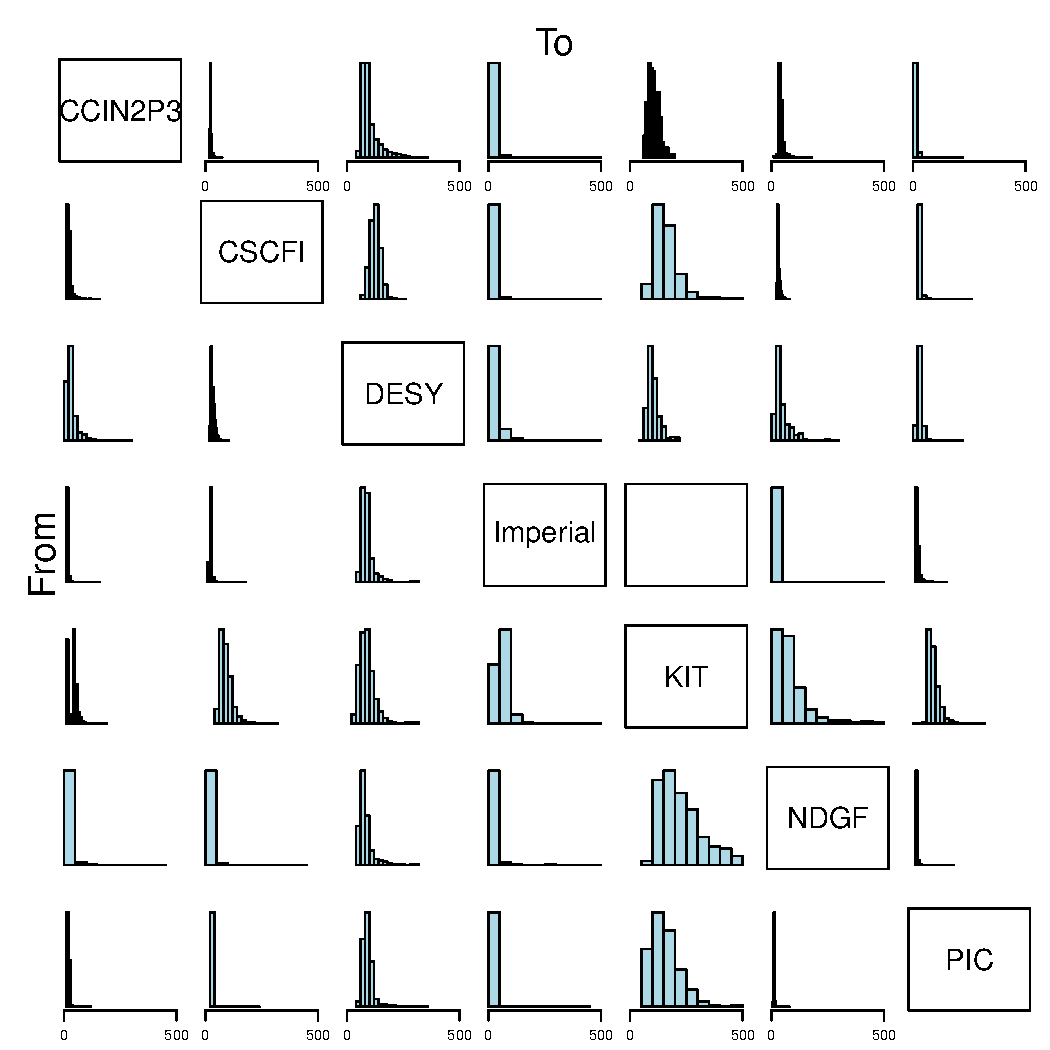
\includegraphics[width=0.8\textwidth]{fts3-mesh.pdf}
       \caption{The FTS3 transfer testbed. Rows show transfers from the named site, columns show transfers to the destination. The horizontal axis for all plots is fixed at 500 seconds, i.e. transfers that proceed at less than 2 MB/sec will overflow.}
 \label{fig:fts3-mesh}
\end{figure}


\subsection{FTS3 server and dCache SE at KIT}
For managing file transfers between sites, an FTS3 instance is setup at KIT. Furthermore, a storage element based on dCache 2.10 on Scientic Linux is created. Both instances are rolled out on physical machines.

\subsubsection{FTS3}
FTS3 supports IPv6 in its baseline version. The service has to bind to IPv6 locally in the FTS3 conguration (IP=::) and to be enabled explicitely for gfal.2 ( IPV6=true). The host is available in the DNS as default dual-host, with IP4 and IPv6 announced in the A and AAAA records, and also with IPv4-only or IPv6-only names with an -ipv4 or -ipv6 appendix, respectively. Thus, all aliases have to included in the host certicate.

File transfers are successfully brokered by the FTS3 instance via IPv4 and IPv6 between the sites. Since most FTS3 instances in production use a separated database instance for performance and failsafe reasons, moving the database to a dedicated machine was tested as well. For the SQL db backends supported by FTS3, IPv6 support had been implemented in MySQL v5.5.3 and MariaDB v5.5.35, which are not available in the baseline SL6 repositories. MariaDB was installed on a dedicated host with version 5.5.42. After binding mysql locally to IPv6 as well ([mysqld] bind-address = ::), the database could be connected remotely with an IPv6-ready mysql client. For the FTS3 service to connect to the remote database via IPv6, the address has to be escaped explicitly, i.e., encapsulating the IP as [IP6]:PORT/fts3 and may depend on the version of the database library used by the FTS3 service.

\subsubsection{dCache based SE}
A dCache instance is setup on a dedicated host. The main hurdle for file transfer access was a reverse lookup by the instance when receiving a file request. After explicitely setting the dual-stack, IPv4-only, and IPv6-only host names in the dCache congfiguration (srm.net.local-hosts=hostname-ipv4,ipv6) and the general hosts file, the storage element is accessible via IPv4 and IPv6 as well.

% Add other sections as appropriate...

\par
\section*{References}

\begin{thebibliography}{1}
\bibitem{ipv6wg} {\tt http://hepix-ipv6.web.cern.ch}
\bibitem{rfc} All Internet Engineering Task Force Requests For Comments (RFC) documents are available
from URLs such as http://www.ietf.org/rfc/rfcNNNN.txt where NNNN is the RFC number, for example {\tt http://www.ietf.org/rfc/rfc2460.txt}
\bibitem{ipv6stat} See for instance {\tt http://www.google.com/ipv6/statistics.html}. The 2\% global connectivity threshold was crossed in September 2013.
\bibitem{rhel} {\tt http://www.redhat.com/products/enterprise-linux/}
\bibitem{cream}
Aiftimiei C, Andreetto P, Bertocco S, Dalla Fina S, Dorigo A,
Frizziero E, Gianelle A, Marzolla M, Mazzucato M, Sgaravatto M,
Traldi S, Zangrando L 2010 Design and Implementation of the gLite CREAM Job
Management Service {\it Future Generation Computer Systems} Volume {\bf 26} Issue
4 pp 654-667, doi: 10.1016/j.future.2009.12.006.
\bibitem{wms}
Cecchi M, Capannini F, Dorigo A, Ghiselli A, Giacomini F, Maraschini M, Marzolla M, Monforte S, Pacini F, Petronzio L, Prelz F 2009 The gLite Workload Management System {\it Advances in Grid and Pervasive Computing: 4th International Conference, GPC}
\bibitem{panda}
Maeno T 2008 PanDA: distributed production and distributed analysis
system for ATLAS {\it J. Phys. Conf. Ser.} {\bf 119} 062036
\bibitem{fts}
Kunszt P, Badino P, Rocha R, Casey J, Frohner A, McCance G 2006 The gLite File Transfer Service
{\it Workshop on Next Generation Distributed Data Management at The Fifteenth IEEE International Symposium on High-Performance Distributed Computing (HPDC2006), Paris, France}
\bibitem{phedgen}
Egeland R, Metson S and  Wildish T 2008 Data transfer infrastructure for
CMS data taking,  {\it XII Advanced Computing and Analysis Techniques in
Physics Research (Erice, Italy: Proceedings of Science)}
\bibitem{cvmfs}
Blomer J et al 2012 Status and future perspectives of CernVM-FS
{\it J. Phys.: Conf. Ser.} {\bf}396 052013
\bibitem{bdii}
Field L and Schulz M W 2004  Grid Deployment Experiences: The path to a production quality LDAP based grid information system {\it Proceedings of the International Conference on Computing in High Energy and Nuclear Physics (CHEP 2004)}
\bibitem{monalisa}
Legrand I, Newman H, Voicu R, Cirstoiu C, Grigoras C, Dobre C, Muraru A,
Costan A, Dediu M and Stratan C 2009 MonALISA: An agent based, dynamic
service system to monitor, control and optimize distributed systems {\it
Computer Physics Communications} Volume {\bf180} Issue 12, December 2009,
Pages 2472–2498
\bibitem{LifeCycle}
    Wildish T 2013 Integration and validation testing for PhEDEx, DBS and DAS with the PhEDEx LifeCycle agent {\it also presented at CHEP 2013}
\bibitem{cms}
The CMS Collaboration 2008 The CMS experiment at the CERN LHC {\it JINST
{\bf 3} S08004}
\bibitem{PhEDEx}
    Egeland R, Wildish T, Metson S 2008 Data transfer infrastructure for CMS data taking {\it XII Advanced Computing and Analysis Techniques in Physics Research (Erice, Italy: Proceedings of Science)}
\bibitem{FTS3}
    Salichos M, Keeble O, Alvarez Ayllon A, Kamil Simon M 2013 FTS3 - Robust, simplified and high-performance data movement service for WLCG {\it also presented at CHEP 2013}
\end{thebibliography}


\end{document}

